\documentclass[14pt, a4 paper]{report}
\usepackage{graphicx} % Required for inserting images
\usepackage{caption}
\usepackage{subcaption}
\usepackage{listings}
\usepackage{amsmath}

\usepackage[utf8]{inputenc}
\usepackage[T1]{fontenc}
\DeclareMathSymbol{\invques}{\mathord}{operators}{`>}
\DeclareUnicodeCharacter{00BF}{\tmquestiondown}
\DeclareRobustCommand{\tmquestiondown}{%
  \ifmmode\invques\else\textquestiondown\fi
}
\usepackage[portuges]{babel}%Babel -- irá activar automaticamente as regras apropriadas de hifenização para a língua todo o
                                   %-- o texto gerado é automaticamente traduzido para Português.
                                   %  Por exemplo, “chapter” irá passar a “capítulo”, “table of contents” a “conteúdo”.
                                   % portuges -- específica para o Português.
\usepackage[utf8]{inputenc} % define o encoding usado texto fonte (input)--usual "utf8" ou "latin1
\usepackage{parcolumns}

\usepackage{graphicx} %permite incluir graficos, tabelas, figuras
\usepackage{url} % para utilizar o comando \url{}
\usepackage{enumerate} %permite escolher, nas listas enumeradas, se os iems sao marcados com letras ou numeros-romanos em vez de numeracao normal

%\usepackage{apalike} % gerar biliografia no estilo 'named' (apalike)

\usepackage{color} % Para escrever em cores
\usepackage{multirow} %tabelas com multilinhas
\usepackage{array} %formatação especial de tabelas em array
\usepackage[pdftex]{hyperref} % transformar as referências internas do seu documento em hiper-ligações.
\usepackage{listings}
\usepackage{xcolor}
\definecolor{codegreen}{rgb}{0,0.6,0}
\definecolor{codegray}{rgb}{0.5,0.5,0.5}
\definecolor{codepurple}{rgb}{0.58,0,0.82}
\definecolor{backcolour}{rgb}{0.95,0.95,0.92}

\lstdefinestyle{mystyle}{
    backgroundcolor=\color{backcolour},   
    commentstyle=\color{codegreen},
    keywordstyle=\color{magenta},
    numberstyle=\tiny\color{codegray},
    stringstyle=\color{codepurple},
    basicstyle=\ttfamily\footnotesize,
    breakatwhitespace=false,         
    breaklines=true,                 
    captionpos=b,                    
    keepspaces=true,                 
    numbers=left,                    
    numbersep=5pt,                  
    showspaces=false,                
    showstringspaces=false,
    showtabs=false,                  
    tabsize=2
}

\lstset{style=mystyle}

%Exemplos de fontes -- nao e vulgar mudar o tipo de fonte
%\usepackage{tgbonum} % Fonte de letra: TEX Gyre Bonum
%\usepackage{lmodern} % Fonte de letra: Latin Modern Sans Serif
%\usepackage{helvet}  % Fonte de letra: Helvetica
%\usepackage{charter} % Fonte de letra:Charter

\definecolor{saddlebrown}{rgb}{0.55, 0.27, 0.07} % para definir uma nova cor, neste caso 'saddlebrown'

\usepackage{listings}  % para utilizar blocos de texto verbatim no estilo 'listings'
%paramerização mais vulgar dos blocos LISTING - GENERAL
\lstset{
	basicstyle=\small, %o tamanho das fontes que são usadas para o código
	numbers=left, % onde colocar a numeração da linha
	numberstyle=\tiny, %o tamanho das fontes que são usadas para a numeração da linha
	numbersep=5pt, %distancia entre a numeração da linha e o codigo
	breaklines=true, %define quebra automática de linha
    frame=tB,  % caixa a volta do codigo
	mathescape=true, %habilita o modo matemático
	escapeinside={(*@}{@*)} % se escrever isto  aceita tudo o que esta dentro das marcas e nao altera
}
%
%\lstset{ %
%	language=Java,							% choose the language of the code
%	basicstyle=\ttfamily\footnotesize,		% the size of the fonts that are used for the code
%	keywordstyle=\bfseries,					% set the keyword style
%	%numbers=left,							% where to put the line-numbers
%	numberstyle=\scriptsize,				% the size of the fonts that are used for the line-numbers
%	stepnumber=2,							% the step between two line-numbers. If it's 1 each line
%											% will be numbered
%	numbersep=5pt,							% how far the line-numbers are from the code
%	backgroundcolor=\color{white},			% choose the background color. You must add \usepackage{color}
%	showspaces=false,						% show spaces adding particular underscores
%	showstringspaces=false,					% underline spaces within strings
%	showtabs=false,							% show tabs within strings adding particular underscores
%	frame=none,								% adds a frame around the code
%	%abovecaptionskip=-.8em,
%	%belowcaptionskip=.7em,
%	tabsize=2,								% sets default tabsize to 2 spaces
%	captionpos=b,							% sets the caption-position to bottom
%	breaklines=true,						% sets automatic line breaking
%	breakatwhitespace=false,				% sets if automatic breaks should only happen at whitespace
%	title=\lstname,							% show the filename of files included with \lstinputlisting;
%											% also try caption instead of title
%	escapeinside={\%*}{*)},					% if you want to add a comment within your code
%	morekeywords={*,...}					% if you want to add more keywords to the set
%}

\usepackage{xspace} % deteta se a seguir a palavra tem uma palavra ou um sinal de pontuaçao se tiver uma palavra da espaço, se for um sinal de pontuaçao nao da espaço

\parindent=2pt %espaço a deixar para fazer a  indentação da primeira linha após um parágrafo
\parskip=4pt % espaço entre o parágrafo e o texto anterior

\setlength{\oddsidemargin}{-1cm} %espaço entre o texto e a margem
\setlength{\textwidth}{18cm} %Comprimento do texto na pagina
\setlength{\headsep}{-1cm} %espaço entre o texto e o cabeçalho
\setlength{\textheight}{23cm} %altura do texto na pagina

% comando '\def' usado para definir abreviatura (macros)
% o primeiro argumento é o nome do novo comando e o segundo entre chavetas é o texto original, ou sequência de controle, para que expande
\def\darius{\textsf{Darius}\xspace}
\def\antlr{\texttt{AnTLR}\xspace}
\def\VM{\href{https://ewvm.epl.di.uminho.pt/}{VM}}
\def\plc{\emph{Processamento de Linguagens e Compiladores}\xspace}
\def\titulo#1{\section{#1}}    %no corpo do documento usa-se na forma '\titulo{MEU TITULO}'
\def\super#1{{\em Supervisor: #1}\\ }
\def\area#1{{\em \'{A}rea: #1}\\[0.2cm]}
\def\resumo{\underline{Resumo}:\\ }
\def\e#1{\emph{#1}}

%\input{LPgeneralDefintions} %permite ler de um ficheiro de texto externo mais definições

\title{Computação Gráfica (3º ano de LCC)\\
       \textbf{Trabalho Prático (Fase 4) — Grupo 3}\\ Relatório de Desenvolvimento}
\author{André Lucena Ribas Ferreira (A94956) 
    \and Carlos Eduardo da Silva Machado (A96936)
    \and Gonçalo Manuel Maia de Sousa (A97485)}
\date{\today} %data

\begin{document}

\maketitle

\begin{abstract}
    Este relatório aborda a solução proposta para o enunciado da 4ª fase do Trabalho Prático da Unidade Curricular "Computação Gráfica". Isto inclui a introdução de iluminação, texturas e cor aos modelos criados. 
\end{abstract}

\tableofcontents

\chapter{Introdução} \label{chap:intro}

O presente relatório tem como objetivo apresentar a solução concebida pelo Grupo 3 para a 4ª fase do Trabalho Prático da Unidade Curricular "Computação Gráfica". 

Esta fase consistiu em implementar normais e coordenadas de textura para cada um dos modelos existentes e integrados nas fases anteriores. Também se atualizou a estrutura aceitável do ficheiro \textit{xml} para poder corresponder tanto a iluminação e a texturas, podendo então ser possível usufruir das mesmas.

À demo desta parte, foi acrescentadas luzes e texturas aos planetas e cores às luas.
\section{Estrutura do Relatório}

Para além deste, o relatório compreende diferentes Capítulos. Em \ref{chap:generator} apresenta-se extensão à implementação da aplicação \textit{generator}. Em \ref{chap:engine} apresenta-se as extensões à implementação da aplicação \textit{engine}. Em \ref{chap:resultado} expõe-se imagens tiradas aos modelos gerados a partir dos \textit{xmls} dos \textit{test files}.
Em \ref{chap:conclusion} apresenta-se a conclusão do relatório.

\chapter{\textit{Generator}} \label{chap:generator}
Neste capítulo, abordamos as mudanças feitas no código relacionado com o \textit{generator}, adicionando funcionalidades pedidas pelo enunciado e alterando o modo como fazíamos algumas operações como a escrita dos pontos em ficheiro. Podemos, então, dividir-los em três partes:

\begin{itemize}
\item IBO's

\item Normais

\item Coordenadas de Textura
\end{itemize}

\section{IBO's}

A implementação mais exigente de \textbf{IBO} junto de normais e de coordenadas de textura implica uma mais preocupada consideração pelos pontos escritos em ficheiro por parte do \textbf{generator}. Nomeadamente, tomamos em consideração todas as faces e vertentes possíveis de cada objeto, tal como a possibilidade de lhe aplicar texturas de modo a dar mais riqueza às cenas. 

Para tal fim, cada um dos pontos foi considerado num espaço de 8 dimensões, com as coordenadas espaciais, as coordenadas do vetor normal e as coordenadas das texturas a ele aplicadas. Qualquer variação de um destes elementos implica a consideração de um novo ponto e, como tal, de um novo indíce adicionado a o \textbf{IBO}.

No ficheiro de modelo \textit{.3d}, foram escritas as coordenadas de posição seguidas das coordenadas normais e das coordenadas de texturas. O número de vértices precede todos estes valores e informa-nos de todos eles.

\section{Normais}

As normais de cada modelo são definidas tendo em consideração cada uma das suas faces, entendendo se os seus vértices devem ser ou não considerados pertencentes a duas faces distintas, de modo a distinguir os elementos da 8ª dimensão, como descrito anteriormente.

\subsubsection{Plane}

Para o \textbf{plane} as normais são dadas facilmente pela orientação do plano, segundo a direção positiva do eixo \textit{yy}, particularmente.

\subsubsection{Box}

As normais da \textbf{box} podem ser feitas de modo análogo ao plano, definindo o vetor normal ao plano de cada uma das faces do cubo.

\subsubsection{Cone}

As normais da base do \textbf{Cone} são trivialmente feitas, as restantes normais são dadas pela rotação do vetor (h, r), após ser normalizado pelo ângulo correto, em que h é a altura do cone e r o raio da base.

\subsubsection{Sphere}

Semelhante à maneira como foram calculados os pontos da esfera os vetors normais são calculados pela rotação de um \textit{array} de vetores à volta do eixo y. Os vetores do \textit{array} são por sua vez calculados por rotação do vetor (0,1,0).

\subsubsection{Cylinder}

As normais das bases do cilindro são feitas trivialmente, além disso, as normais do corpo do cilindro são feitas por rotação de um vetor paralelo ao eixo z.

\subsubsection{Torus}

As normais do cone são feitas de modo análogo à esfera.
São gerados os vetores de um círculo e este é rodado à volta do eixo y.

\section{Coordenadas de Textura}

\subsubsection{Plane}

As coordenadas de textura do plano são diretamente retiradas das subdivisões dos eixos.

\subsubsection{Box}

As coordenadas de textura do cubo são feitas mapeando a textura em todas as faces do cubo, tratando cada uma como um plano próprio.

\subsubsection{Cone}

No caso do cone a textura é mapeada sobre a superfície. De modo que quanto mais próximo do topo do cone mais comprimida é a textura.
É importante notar que os pontos do topo do cone bem como os pontos da "borda" são repetidos.

\subsubsection{Sphere}

As coordenadas de textura da esfera são feitas da mesma maneira do cone.
Neste caso os pontos do topo e a base da esfera são repetidos.

\chapter{\textit{Engine}} \label{chap:engine}

Neste capítulo, vamos abordar as mudanças que fizemos ao código relativo ao \textit{engine} de modo a suprir as novas necessidades enunciadas na fase 4 e alguns extras.

Deste modo, vamos dividir este capítulo em:

\begin{itemize}

\item Normais e Texturas
\item Luzes e Cores
\item Mipmapping

\end{itemize}

\section{Normais e Texturas}

A implementação do \textbf{IBO} do lado da \textit{engine} baseia-se em conseguir ler corretamente do ficheiro as coordenadas corretas e de as associar corretamente ao seu lugar dentro de cada um dos \textbf{VBO's} definidos, tal como na fase passada se fez apenas com as coordenadas dos pontos. Desse modo, geraram-se dois novos \textbf{VBO's} e associaram-se-lhe as semânticas próprias de cada um. A leitura continua a ocorrer a partir do ficheiro de modelos, que verifica se o modelo já foi lido ou não, colocando apenas um de cada instância do modelo no \textbf{VBO}, repetindo apenas os índices. 

\begin{lstlisting}[language = c++]
unsigned int before = points->size();
points->resize(before + n);
normals->resize(before + n);
texCoords->resize(2*before/3 + 2*n/3);
filestream.read((char*)(points->data() + before), sizeof(float) * n);
filestream.read((char*)(normals->data() + before), sizeof(float) * n);
filestream.read((char*)(texCoords->data() + 2*before/3), sizeof(float) * 2*n/3);

unsigned int n_indices;
filestream.read((char*)&n_indices, sizeof(unsigned int));
//printf("%d\n", n_indices);
unsigned int* indices_buf = (unsigned int*)malloc(sizeof(unsigned int) * n_indices);
filestream.read((char*)(indices_buf), sizeof(unsigned int) * n_indices);
\end{lstlisting}

Uma característica importante  das texturas está na expansão da classe \textbf{Model}, que necessita que se lhe associe o \textit{char} correspondente à textura que foi carregada, quando encontrada no \textit{xml}. Cada modelo saberá qual a sua textura e, no momento de desenho, esta é carregada e utilizada.

\begin{lstlisting}[language = c++]
glBindTexture(GL_TEXTURE_2D, groupModel->texID);
glBindBuffer(GL_ARRAY_BUFFER, buffer[0]);
glVertexPointer(3, GL_FLOAT, 0, 0);
\end{lstlisting}

\section{Luzes e Cores}

Para guardar os três tipos de luzes criamos 3 tipos de classes diferentes que herdam da mesma classe \textit{Lights}, essas classes são: \textit{Point, Directional e Spotlight}. A classe \textit{Point} e \textit{Directional} têm o mesmo principio, o que apenas muda é o facto de o quarto argumento no primeiro ser 1 e no segundo ser 0, pois a coordenada w num ponto é 1 e num vetor é 0. A \textit{Spotlight} vai conter um \textit{array} que representa o ponto, um vetor que representa a direção e um \textit{cutoff} que especifica o ângulo de propagação máximo da luz. Além disso, existe uma instância \textit{GLuint} \textit{number} que indica qual a luz que é, ou seja, se for a primeira terá o valor de \textit{GL\_LIGHT0}, isso permite que ao chamar a função \textit{getNumber} nos dê qual a luz que o objeto indica. Além disso, temos o método \textit{drawLight} que quando executado utiliza as funções do \textit{opengl} indicadas para aquele tipo de luz.

\begin{lstlisting}[language=c++]
void Spotlight::drawLight() {
    glLightfv(number, GL_POSITION, point);
    glLightfv(number, GL_SPOT_DIRECTION, dir);
    glLightfv(number, GL_SPOT_CUTOFF, &cutoff);
}

void Point::drawLight() {
    glLightfv(GL_LIGHT0, GL_POSITION, point);
}

void Directional::drawLight() {
    glLightfv(number, GL_POSITION, point);
}

GLuint Point::getNumber(){
    return Point::number;
}

GLuint Directional::getNumber(){
    return Directional::number;
}

GLuint Spotlight::getNumber(){
    return Spotlight::number;
}
\end{lstlisting}

Como podemos ver no código acima demonstrado, aplicamos \textit{glLightfv} com \textit{GL\_POSITION} tanto para a classe \textit{Point} quanto para a classe \textit{Directional}, já a \textit{Spotlight} temos de fazer \textit{glLightfv} de acordo com as instâncias acima mencionas.

Deste modo, além do \textit{glEnable(GL\_LIGHTING} para ativar as luzes, e aplicar \textit{GL\_LIGHT\_MODEL\_AMBIENT} para a cor ambiente, aplicamos o seguinte ciclo uma vez antes do main loop, de modo a inicializar as luzes:

\begin{lstlisting}[language = c++]
if (!lights->empty()) glEnable(GL_LIGHTING);
	for(Light* light: *lights){
		glEnable(light->getNumber());
		glLightfv(light->getNumber(), GL_AMBIENT, light->ambient);
		glLightfv(light->getNumber(), GL_DIFFUSE, light->diffuse);
		glLightfv(light->getNumber(), GL_SPECULAR, light->specular);
	}
\end{lstlisting}

Depois, na função \textit{renderScene} fazemos:
\begin{lstlisting}[language = c++]
for(Light* light: *lights){
    light->drawLight();
}
\end{lstlisting}
Para ajustar a luz, pois a mesma poderá ser afetada pelas transformações geométricas e precisamos de a ajustar.

O \textit{parsing} do ficheiro \textit{xml} para o caso das luzes ficará numa nova função:

Temos a opção no \textit{xml} de adicionar com às componentes de cada luz e de colocar, ou não luz ambiente global.
\begin{lstlisting}[language = c++]
void parse_lights(xml_node<> *lights_node, vector<Light*>* lights, float* amb, int* amb_active){
    xml_node<> *temp;
    xml_attribute<> *attr;
    GLuint numbers[] = {GL_LIGHT0, GL_LIGHT1, GL_LIGHT2, GL_LIGHT3, GL_LIGHT4, GL_LIGHT5, GL_LIGHT6, GL_LIGHT7};
    int number = 0;
    if((temp = lights_node->first_node("amb"))){
        if((attr = temp->first_attribute("active"))){
            if(!strcmp(attr->value(), "false")){
                amb_active = 0;
            }

            if((attr = temp->first_attribute("R"))){
                amb[0] = atof(attr->value())/255;
            }

            if((attr = temp->first_attribute("G"))){
                amb[1] = atof(attr->value())/255;
            }

            if((attr = temp->first_attribute("B"))){
                amb[2] = atof(attr->value())/255;
            }
        }
    }
    for(temp = lights_node->first_node("light"); number < 8 && temp; temp = temp->next_sibling("light"), number++){
        if((attr = temp->first_attribute("type")) && !strcmp(attr->value(), "point")){
            Point* point = new Point();
            if((attr = temp->first_attribute("posx")))
                point->point[0] = atof(attr->value());
        
            if((attr = temp->first_attribute("posy")))
                point->point[1] = atof(attr->value());
        
            if((attr = temp->first_attribute("posz")))
                point->point[2] = atof(attr->value());

            point->point[3] = 1.0;

            point->number = numbers[number];
            lights->push_back(point);
        } else if((attr = temp->first_attribute("type")) && !strcmp(attr->value(), "directional")){
            Directional* directional = new Directional();
            if((attr = temp->first_attribute("dirx")))
                directional->point[0] = atof(attr->value());
        
            if((attr = temp->first_attribute("diry")))
                directional->point[1] = atof(attr->value());
        
            if((attr = temp->first_attribute("dirz")))
                directional->point[2] = atof(attr->value());

            directional->point[3] = 0.0;

            //printf("%f %f %f\n", directional->point[0], directional->point[1], directional->point[2]);

            directional->number = numbers[number];
            lights->push_back(directional);
        } else if((attr = temp->first_attribute("type")) && !strcmp(attr->value(), "spotlight")){
            Spotlight* spotlight = new Spotlight();
            if((attr = temp->first_attribute("posx")))
                spotlight->point[0] = atof(attr->value());
        
            if((attr = temp->first_attribute("posy")))
                spotlight->point[1] = atof(attr->value());
        
            if((attr = temp->first_attribute("posz")))
                spotlight->point[2] = atof(attr->value());

            spotlight->point[3] = 1.0;
        
            if((attr = temp->first_attribute("dirx")))
                spotlight->dir[0] = atof(attr->value());
        
            if((attr = temp->first_attribute("diry")))
                spotlight->dir[1] = atof(attr->value());
        
            if((attr = temp->first_attribute("dirz")))
                spotlight->dir[2] = atof(attr->value());

            if((attr = temp->first_attribute("cutoff")))
                spotlight->cutoff = atof(attr->value());
            spotlight->number = numbers[number];
            lights->push_back(spotlight);
        }
        
        if(temp->first_node("color")){
            xml_node<> *tempColor;
            xml_attribute<> *tempAttr;
            if((tempColor = temp->first_node("diffuse"))){
                if((tempAttr = tempColor->first_attribute("R"))){
                    lights->at(number)->diffuse[0] = atof(tempAttr->value())/255;
                }

                if((tempAttr = tempColor->first_attribute("G"))){
                    lights->at(number)->diffuse[1] = atof(tempAttr->value())/255;
                }

                if((tempAttr = tempColor->first_attribute("B"))){
                    lights->at(number)->diffuse[2] = atof(tempAttr->value())/255;
                }
            }

            if((tempColor = temp->first_node("ambient"))){
                if((tempAttr = tempColor->first_attribute("R"))){
                    lights->at(number)->ambient[0] = atof(tempAttr->value())/255;
                }

                if((tempAttr = tempColor->first_attribute("G"))){
                    lights->at(number)->ambient[1] = atof(tempAttr->value())/255;
                }

                if((tempAttr = tempColor->first_attribute("B"))){
                    lights->at(number)->ambient[2] = atof(tempAttr->value())/255;
                }
            }

            if((tempColor = temp->first_node("specular"))){
                if((tempAttr = tempColor->first_attribute("R"))){
                    lights->at(number)->specular[0] = atof(tempAttr->value())/255;
                }

                if((tempAttr = tempColor->first_attribute("G"))){
                    lights->at(number)->specular[1] = atof(tempAttr->value())/255;
                } 

                if((tempAttr = tempColor->first_attribute("B"))){
                    lights->at(number)->specular[2] = atof(tempAttr->value())/255;
                }
            }
        }
    }
}
\end{lstlisting}

É feito da mesma maneira que outros nodos do \textit{xml}, com o detalhe que temos um \textit{array} com os \textit{GLuints} das luzes e são atribuídas às luzes pela ordem do \textit{xml}.

Em relação aos modelos, fazemos o \textit{parsing} da seguinte maneira:

\begin{lstlisting}[language = c++]
if((temp = node_models->first_node("color"))){
            xml_node<> *tempColor;
            xml_attribute<> *tempAttr;
            if((tempColor = temp->first_node("diffuse"))){
                if((tempAttr = tempColor->first_attribute("R"))){
                    model->diffuse[0] = atof(tempAttr->value())/255;
                }

                if((tempAttr = tempColor->first_attribute("G"))){
                    model->diffuse[1] = atof(tempAttr->value())/255;
                }

                if((tempAttr = tempColor->first_attribute("B"))){
                    model->diffuse[2] = atof(tempAttr->value())/255;
                }
            }

            if((tempColor = temp->first_node("ambient"))){
                if((tempAttr = tempColor->first_attribute("R"))){
                    model->ambient[0] = atof(tempAttr->value())/255;
                }

                if((tempAttr = tempColor->first_attribute("G"))){
                    model->ambient[1] = atof(tempAttr->value())/255;
                }

                if((tempAttr = tempColor->first_attribute("B"))){
                    model->ambient[2] = atof(tempAttr->value())/255;
                }
            }

            if((tempColor = temp->first_node("specular"))){
                if((tempAttr = tempColor->first_attribute("R"))){
                    model->specular[0] = atof(tempAttr->value())/255;
                }

                if((tempAttr = tempColor->first_attribute("G"))){
                    model->specular[1] = atof(tempAttr->value())/255;
                } 

                if((tempAttr = tempColor->first_attribute("B"))){
                    model->specular[2] = atof(tempAttr->value())/255;
                }
            }

            if((tempColor = temp->first_node("emissive"))){
                if((tempAttr = tempColor->first_attribute("R"))){
                    model->emissive[0] = atof(tempAttr->value())/255;
                }

                if((tempAttr = tempColor->first_attribute("G"))){
                    model->emissive[1] = atof(tempAttr->value())/255;
                }

                if((tempAttr = tempColor->first_attribute("B"))){
                    model->emissive[2] = atof(tempAttr->value())/255;
                }
            }

            if((tempColor = temp->first_node("shininess"))){
                if((tempAttr = tempColor->first_attribute("value"))){
                    model->shininess = atof(tempAttr->value());
                }
            }
        }
\end{lstlisting}
Dividimos cada componente por 255 de modo a garantir que os valores fiquem entre 0 e 1. Caso não haja o nodo \textit{Color} no \textit{xml}, ou alguma das componentes não for indicada tomamos com padrão os valores dados pelo unciado. A classe \textit{Model} terá no seu interior as seguintes instâncias:

\begin{lstlisting}
    float diffuse[4] = {200, 200, 200, 1.0};
    float ambient[4] = {50, 50, 50, 1.0};
    float specular[4] = {0, 0, 0, 1.0};
    float emissive[4] = {0, 0, 0, 1.0};
    GLfloat shininess = 0;
\end{lstlisting}

Para cada modelo, antes de efetivamente desenha-lo, indicamos as luzes do objeto com as funções \textit{glMaterialfv} e \textit{glMaterialf}:

\begin{lstlisting}[language = c++]
    glMaterialfv(GL_FRONT, GL_SPECULAR, groupModel->specular);
	glMaterialfv(GL_FRONT, GL_AMBIENT, groupModel->ambient);
    glMaterialfv(GL_FRONT, GL_DIFFUSE, groupModel->diffuse);
    glMaterialfv(GL_FRONT, GL_EMISSION, groupModel->emissive);
    glMaterialf(GL_FRONT, GL_SHININESS, groupModel->shininess);
\end{lstlisting}

\section{Mipmapping}
Adicionamos \textit{Mipmapping} com a \textit{flag} \textit{GL\_LINEAR\_MIPMAP\_LINEAR} o que faz com que algumas imagens do exemplo fiquem ligeiramente diferentes por causa da interpolação.

\chapter{Resultados} \label{chap:resultado}

Neste capítulo apresentamos os resultados obtidos da execução de ambas as aplicações utilizando os ficheiros de teste fornecidos.

\begin{figure}[h]
    \centering
    \begin{subfigure}{.5\textwidth}
    \centering
    \includegraphics[width=0.9\linewidth]{4_1.png}
    \caption{Teste 1}
    \label{fig:sub1}
    \end{subfigure}%
    \begin{subfigure}{.5\textwidth}
    \centering
    \includegraphics[width=0.9\linewidth]{4_2.png}
    \caption{Teste 2}
    \label{fig:sub2}
    \end{subfigure}%
    \\
    \begin{subfigure}{.5\textwidth}
    \centering
    \includegraphics[width=0.9\linewidth]{4_3.png}
    \caption{Teste 3}
    \label{fig:sub3}
    \end{subfigure}%
    \begin{subfigure}{.5\textwidth}
    \centering
    \includegraphics[width=0.9\linewidth]{4_4.png}
    \caption{Teste 4}
    \label{fig:sub4}
    \end{subfigure}%
    \label{fig:2}
\end{figure}
\begin{figure}
    \begin{subfigure}{.5\textwidth}
    \centering
    \includegraphics[width=0.9\linewidth]{4_5.png}
    \caption{Teste 5}
    \label{fig:sub5}
    \end{subfigure}%
    \begin{subfigure}{.5\textwidth}
    \centering
    \includegraphics[width=0.9\linewidth]{4_6.png}
    \caption{Teste 6}
    \label{fig:sub6}
    \end{subfigure}%
    \label{fig:2}
\end{figure}

\section{Demo}

A Demo foi estendida acrescentando texturas a cada um dos planetas principais e à lua da Terra, tal como foram acrescentadas luzes e cor emissiva ao Sol para emular a iluminação e as sombras emitidas. Também foram dadas cores a cada um dos restantes corpos celestes, incluindo do cometa. Foi também corrigida a trajetória da elipse do cometa para ser mais circular.

\begin{figure}[h]
    \centering
    \begin{subfigure}{.5\textwidth}
    \centering
    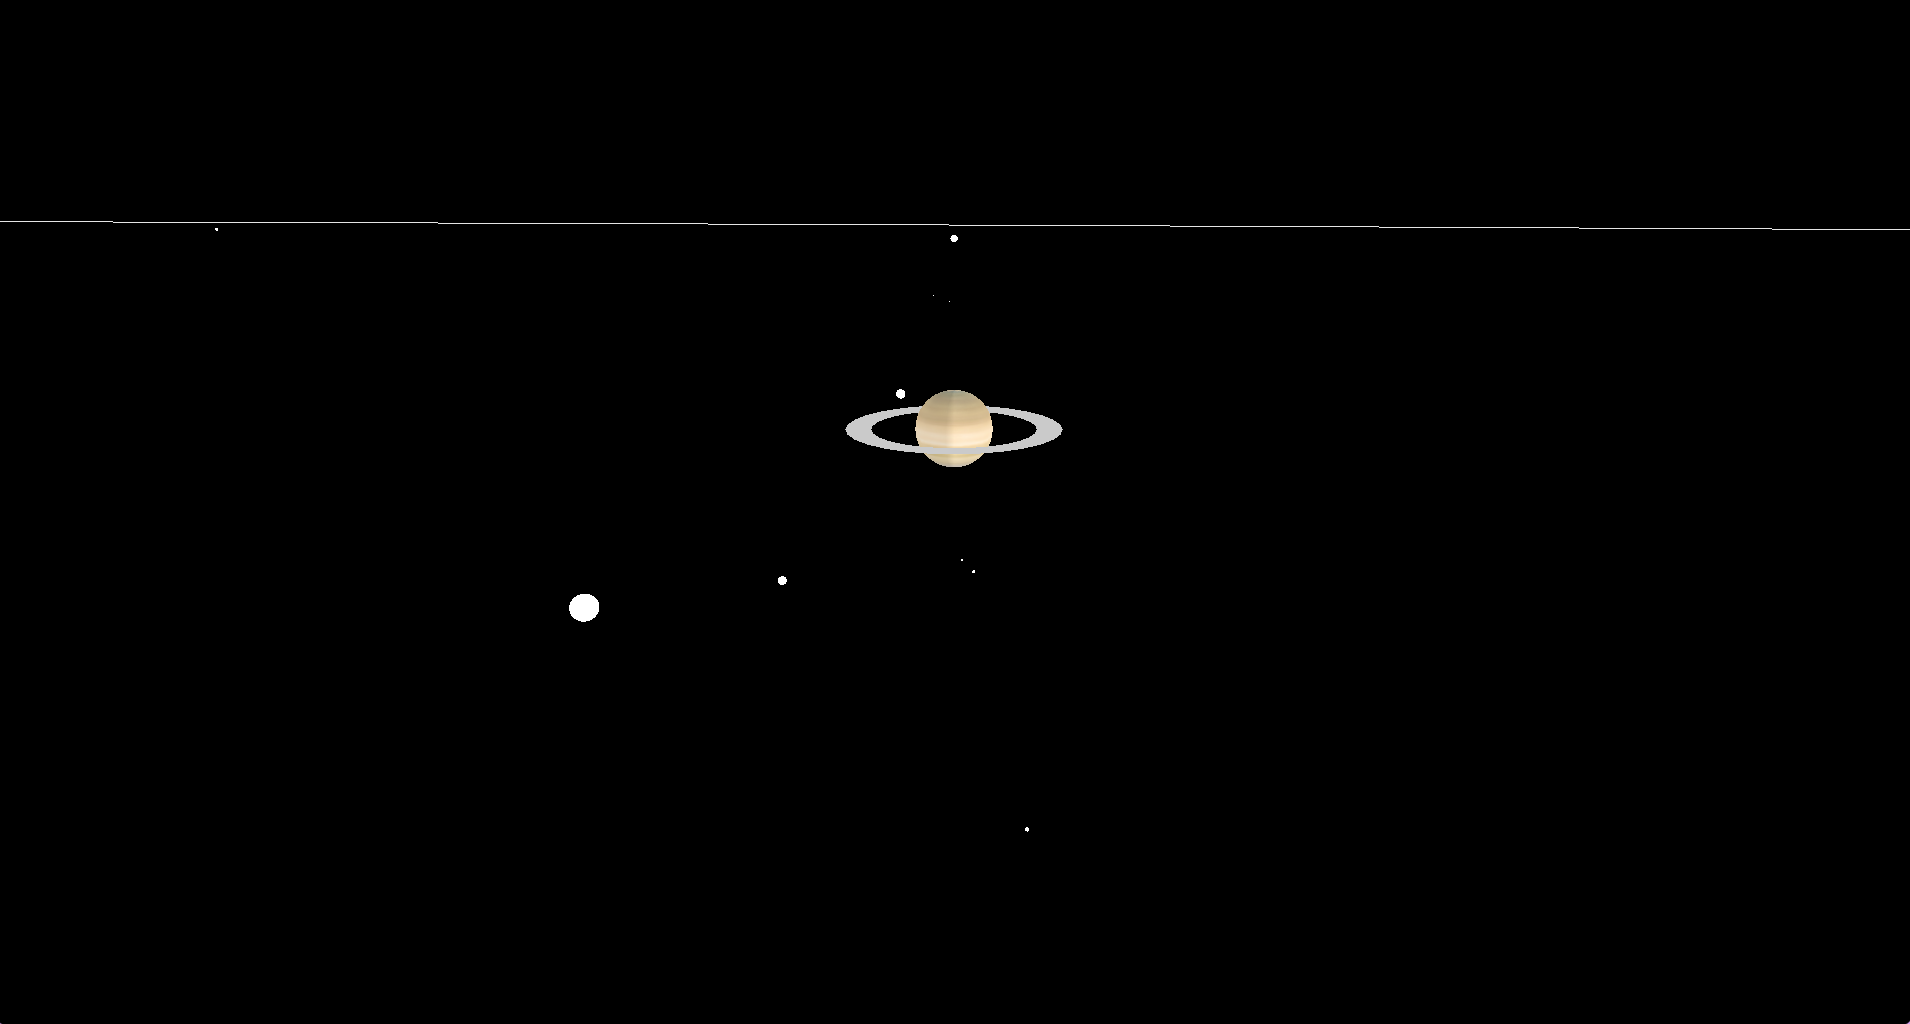
\includegraphics[width=0.9\textwidth]{saturn_midle.png}
    \caption{Saturno}
    \label{fig:sub5}
    \end{subfigure}%
    \begin{subfigure}{.5\textwidth}
    \centering
    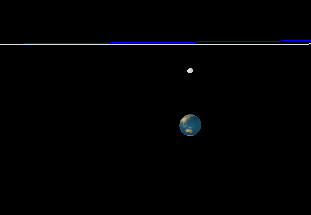
\includegraphics[width=0.9\textwidth]{earth.png}
    \caption{Terra}
    \label{fig:sub6}
    \end{subfigure}%
    \\
\end{figure}
\begin{figure}[h]
    \begin{subfigure}{.5\textwidth}
    \centering
    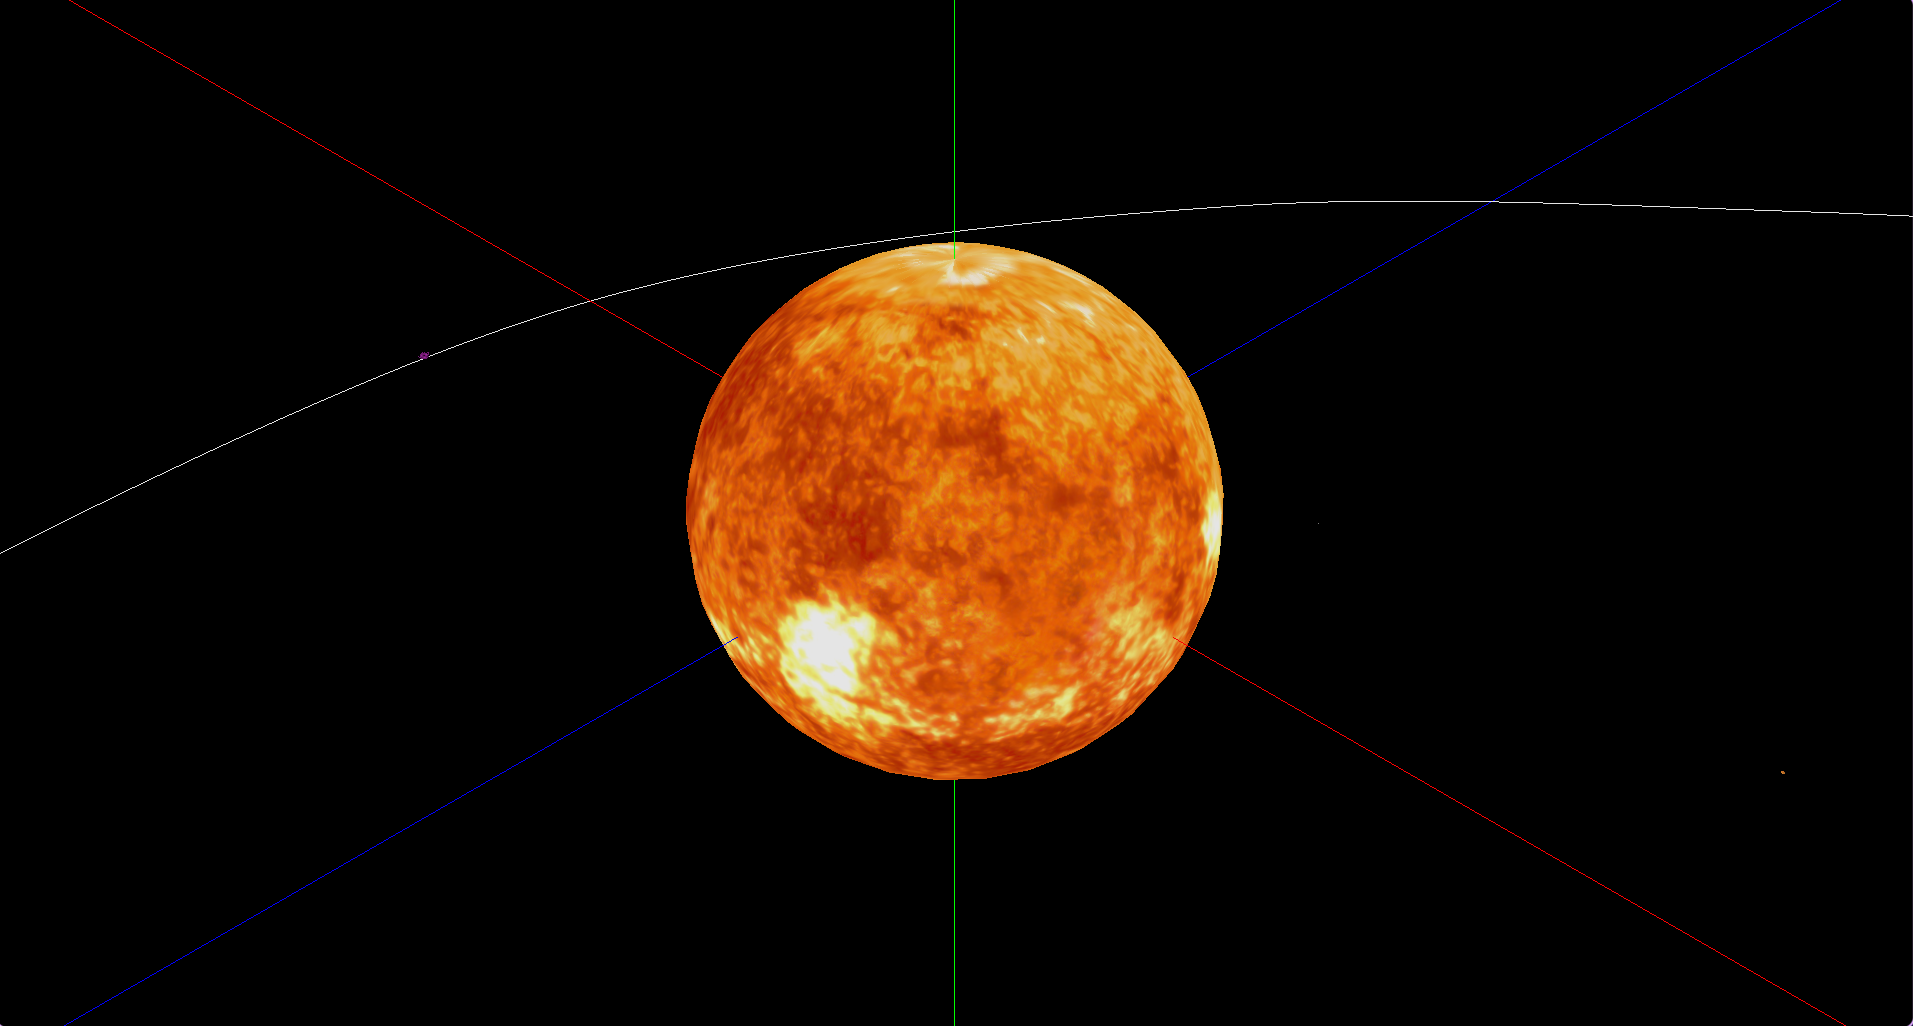
\includegraphics[width=0.9\textwidth]{sun_tex.png}
    \caption{Sol}
    \label{fig:sub5}
    \end{subfigure}%
    \begin{subfigure}{.5\textwidth}
    \centering
    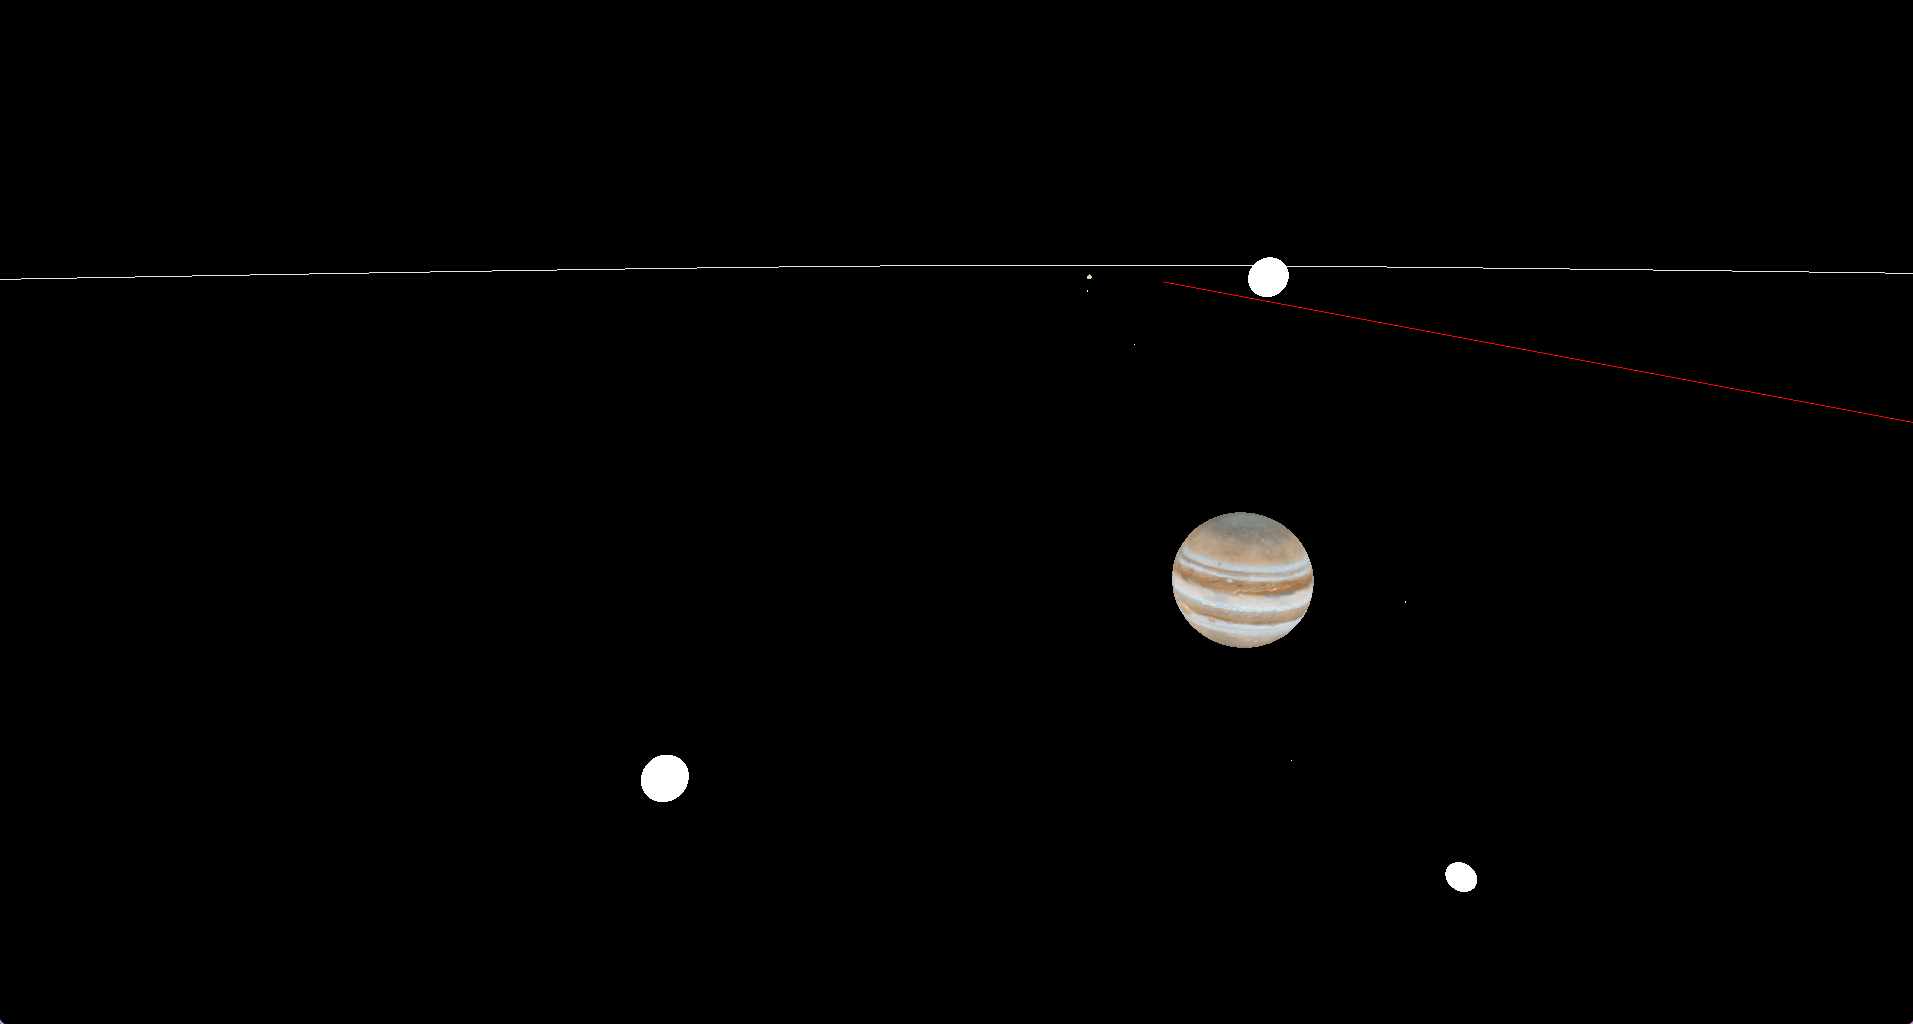
\includegraphics[width=0.9\textwidth]{jupyter_front.png}
    \caption{Júpiter}
    \label{fig:sub6}
    \end{subfigure}%
    \label{fig:2}
\end{figure}

\chapter{Conclusão} \label{chap:conclusion}
Em suma, ao longo deste relatório foi implementada a funcionalidade de cores e de texturas. Também foi implementada a capacidade de adicionar luzes à cena. O desenho das primitivas foi potenciado pela utilização de \textbf{IBO's} ao ponto de se conseguir reduzir o número de chamadas aos \textit{drivers} e categorizar corretamente cada m dos pontos. Por fim, a demo foi aumentada para incluir luzes e texturas e espelhar assim os nossos avanços.

\end{document}

